\begin{exercise}{Détermination d'un produit de solubilité par titrage redox}{2}{PCSI}{Chimie générale, Réactions de précipité, Oxydoréduction, Titrage}{chocron}

On souhaite déterminer la constante de solubilité de l'iodure de plomb par titrage redox.


\begin{questions}
\questioncours Discuter de l'influence de la précipitation sur la valeur du potentiel standard d'un couple redox.


\begin{EnvUplevel}
Étude préliminaire : dosage des ions iodure par le cérium(IV) en milieu chlorure. 
On dose 100 mL d'une solution de I$^-$ à la concentration 1,0$\cdot$10$^{-3}$ mol.L$^{-1}$ par une solution de Ce$^{4+}$ à 0,050 mol.L$^{-1}$, en présence d'ions chlorure dont la concentration peut être supposée constante et égale à 1 mol.L$^{-1}$.

\end{EnvUplevel}

\question Donner les degrés d'oxydation de l'iode dans les trois espèces considérées.

\question Montrer qu'on peut prévoir deux réactions successives pour ce dosage. Calculer les constantes d'équilibres de ces réactions et les volumes équivalents correspondants. 

\question On suit ce dosage par potentiométrie : préciser les électrodes à utiliser. 

\begin{EnvUplevel}
Pour déterminer le produit de solubilité de PbI$_2$, on prépare une solution saturée d'iodure de plomb. On prélève 50 mL de la solution surnageante que l'on verse dans un bécher et on ajoute 50 mL d'acide chlorhydrique concentré.
On effectue le dosage par une solution de cérium(IV) à 0,048 mol.L$^{-1}$ avec un suivi potentiométrique :
\end{EnvUplevel}

\begin{figure}[H]
    \centering
    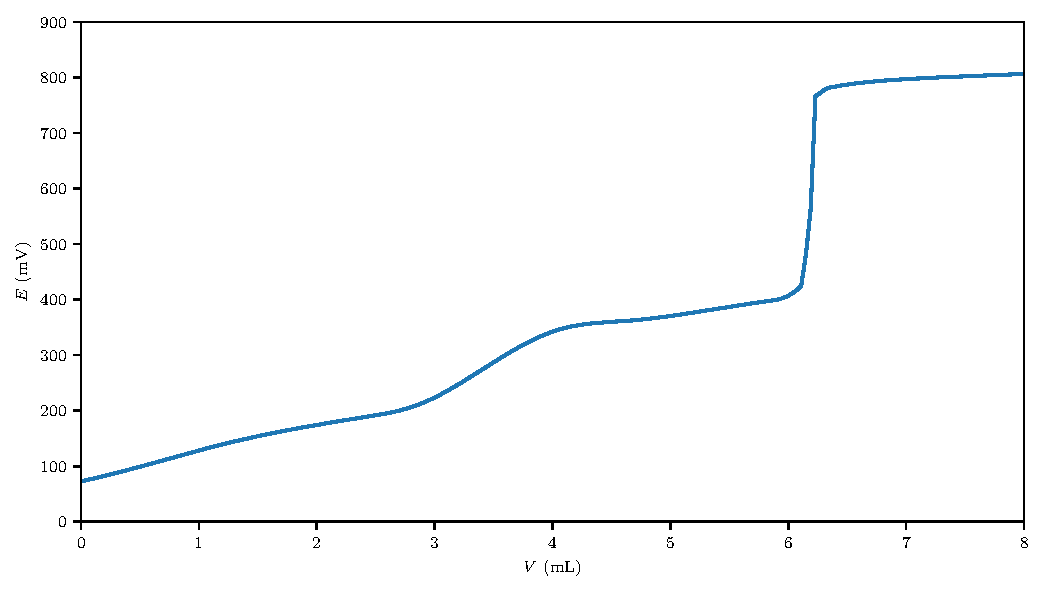
\includegraphics[width=\linewidth]{chimiePC/gene/dosage_redox.pdf}\vspace{-1em}
    \caption{Dosage potentiométrique de la solution par les ions cérium Ce$^{4+}$.}
\end{figure}

\question En déduire la valeur du produit de solubilité de l'iodure de plomb. 

\question Discuter l'intérêt de se placer en milieu chlorure pour ce dosage.
\end{questions}

\paragraph{Données : } potentiels standards $E^\circ$ dans les CNTP
\begin{center}\begin{tabularx}{.7\linewidth}{rCCC}
    \hline
    & $\mathrm{{IC\ell_2^-}_{(aq)} \,/\, {I_2}_{(aq)}}$ & $\mathrm{{I_2}_{(aq)} \,/\, {I^-_{}}_{(aq)}}$ & $\mathrm{{Ce^{4+}}_{(aq)} \,/\, {Ce^{3+}}_{(aq)}}$ \\
    $E^\circ$ (V) & 1,15 & 0,62 & 1,44 \\ \hline\hline 
\end{tabularx}
\end{center}

On note: $e^\circ = \dfrac{RT}{\scr{F}} \ln10 = 59$ mV.

\end{exercise}

\begin{solution}

\begin{questions}
\questioncours
 On considère un couple redox $Ox/Red$ tel que $Ox + ne^- = Red$ (1).
 
 On suppose que l'oxydant peut précipiter selon l'équilibre Ox + mX $\rightleftarrows OxX_{m(s)}$ avec $K_s=[Ox]\times[X]^m$
 
 On considère le nouveau couple redox $OxX_m/Red$ tel que $OxX_m + ne^- = Red + mX $   (2).
 
 La formule de Nerst donne $E_1 = E^\circ(Ox/Red) + \frac{0,06}{n}log(\frac{[Ox]}{[Red]})$ et $E_2 = E^\circ(OxX_m/Red) + \frac{0,06}{n}log(\frac{1}{[Red][X]^m})$.
 
A l'équilibre entre toutes ces espèces, les potentiels sont égaux. Cela donne donc $E^\circ(OxX_m/Red) = E^\circ(Ox/Red) - \frac{0,06}{n}pK_s $

Ainsi, lorsque l'oxydant peut précipiter, le potentiel standard du nouveau couple est abaissé et l'oxydant est donc moins réactif. De la même manière, lorsque le réducteur peut précipiter, on montre que le potentiel standard du nouveau couple augmente de $\frac{0,06}{n}pK_s$ par rapport à celui du couple $Ox/Red$ ce qui signifie également que le réducteur est moins réactif. 


\question I$^-$ : D.O.${} = -$I

I$_2$ : D.O.${} = 0$

IC$\ell_2^-$ : C$\ell$ est plus électronégatif que I donc son D.O. est de $-$I. On a donc $x-2\times1 = -1$ d'où D.O.${} = +$I.

\question La première réaction de dosage est
\begin{equation}
    \mathrm{2I^- + 2Ce^{4+} \longrightarrow I_2 + 2Ce^{3+}}, \tag{1}
\end{equation}
dont la constante est
$$\log(K_1) = 2 \times\dfrac{E^\circ\qty\big(\mathrm{Ce^{4+} / Ce^{3+}}) - E^\circ\qty\big(\mathrm{I_2 /I^-})}{e^\circ} = 27,3.$$

\`A l'équivalence, $\mathrm{[I^-]} \times V_\text{tot} = \mathrm{[Ce^{4+}]} \times V_\text{eq1}$, d'où $V_\text{eq1} = 2,0$ mL. 

Or, le bécher contenant Ce$^{3+}$, I$_2$ et C$\ell^-$, si on continue d'ajouter des ions cérium(IV), le diiode formé va réagir avec les ions Ce$^{4+}$, selon la réaction
\begin{equation}
    \mathrm{I_2 + 2Ce^{4+} + 4 C\ell^- \longrightarrow 2 IC\ell_2^- + 2Ce^{3+}}, \tag{2}
\end{equation}
avec
$$\log(K_2) = 2 \times\dfrac{E^\circ\qty\big(\mathrm{Ce^{4+} / Ce^{3+}}) - E^\circ\qty\big(\mathrm{IC\ell_2^- /I_2})}{e^\circ} = 9,70,$$
et à la deuxième équivalence, $\mathrm{[I_2]} \times V_\text{tot} = \dfrac{1}{2} \times \mathrm{[Ce^{4+}]} \times \qty\big(V_\text{eq2} - V_\text{eq1})$. Or I$_2$ est formé par la première réaction de dosage donc [I$_2$]=$\frac{[\text{I}^-]}{2}$. On a donc $V_\text{eq2} = 2 \times V_\text{eq1} = 4,0$ mL.

\question On utilise deux électrodes : une électrode de mesure (en général en platine, métal inerte puisque toutes les espèces sont en solution) et une électrode de référence (électrode au calomel saturé par exemple).

\question Dans la solution saturée, 
$$\mathrm{PbI_2 \rightleftarrows Pb^{2+} + 2I^-},$$
avec [Pb$^2+] = s$ et [I$^-] = 2s$. On a donc $K_s$=[Pb$^{2+}$]$\times$[I$^-]^2 = 4s^3$.

D'après la courbe de dosage de la solution, $V_\text{eq2} = 6,6$ mL donc $V_\text{eq1} = 3,3$ mL.

On a donc [I$^-] = 3,2 \times 10^{-3}$ mol$\cdot$L$^{-1}$.

D'où $K_s = 1,6 \times 10 ^{-8}$.

\question On remarque sur la courbe de dosage que la première équivalence n'est pas très lisible. La détermination du produit de solubilité a été faite par exploitation de la deuxième équivalence.


En l'absence des ions chlorure, seule la première équivalence aurait eu lieu et le dosage aurait été peu exploitable.

Par ailleurs, l'utilisation d'acide chlorhydrique concentré permet d'éviter la formation d'hydroxydes de plomb.

\end{questions}


\end{solution}















